\chapter{Mathematical Models of Identifying Sections}

\section{DataModification}

\subsection{DataModel}

\subsection{Smoothing}

\subsection{Savitzky-Golay Filtering}

\newpage
\section{Section Identification}
The following section will describe the solution for the identification of sections. And is split into two parts. The first explains the rough identification of sections. These sections will then be given to a classification method that clearly identifies the type of section, be it a curve or a straight line. 

\subsection{Identification}
The identification is split into three parts that will be executed serial. After smoothing and filtering of the dataset. The x-axis acceleration values will be split into two groups. This split is happening with a singular x value representing a threshold. In the positive and negative acceleration range. A visual representation of the threshold can be seen in figure \ref{upperlowerBound}. in this case, the threshold is set to 3.5. All points below the lower bound and above the upper bound will be grouped inside a dataset, while all the points in between are grouped in another.
\begin{figure}[H]
	\centering
	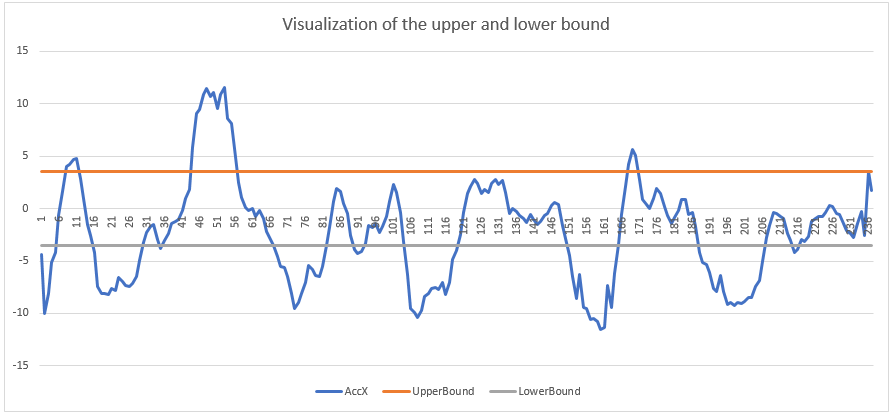
\includegraphics[scale= 0.6]{Pictures/upperandlowerbound.png}
	\caption{Visualization of the thresholds for the upper and lower dataset}
	\label{upperlowerBound}
\end{figure}
After separating the datasets with the threshold, the points above the threshold are considered as expected curves. Therefore it is cleaned in a second step. Because a curve cannot be created with only one point above the threshold, single points will be put back into the dataset in between the thresholds. The last step is grouping the points into sections. The points in between are created as new sections with ten points. A section, that is above the threshold will be created with the first point above and the last point above.

\subsection{Classification}

\section{Section Rating}
Because the focus of our project was the identification of sections, the section rating part contains a simple implementation. The core principle is determining the fastest lap and comparing the time footprint of the other sections to the sections of the fastest lap.